\chapter{Sustainability Approach}  % Better not to put 'airy' stuff like The \textit{Swing}: a Sustainable Concept in chapter titles of a scientific document
\label{ch:Sustainability_Approach}
The \textit{Swing} aims to revolutionise the transportation industry by providing a sustainable alternative to traditional ground transportation.
In the face of the urgent challenges posed by climate change, with approximately 24\% of global carbon emissions attributed to the transportation sector \cite{CO2Transport}, it is crucial to assess the environmental impact of this innovative vehicle.
Evaluating the \textit{Swing}’s sustainability is essential to ensure it contributes positively to reducing the carbon footprint and promoting a greener future for urban mobility. In this chapter, the energy consumption of the \textit{Swing} will be compared to that of competitors (\Cref{sec:energyconsumption}); the impact of the vehicle on urban environments is then considered in \Cref{sec:urbanimpact}; \Cref{sec:emissionsevaluation} covers a qualitative evaluation of the emissions; finally, the reusability requirements are addressed in \Cref{sec:reusability}.



\section{Energy Consumption}
\label{sec:energyconsumption}
Firstly, it is important to acknowledge that the \textit{Swing} is a fully electric vehicle that utilises renewable energy sources, such as solar and wind, for most of its power.
This commitment to renewable energy places the \textit{Swing} ahead of the vast majority of current ground and air transport options, According to the International Energy Agency (IEA), as of 2023, approximately 95\% of the world’s transportation sector continues to rely on fossil fuels.

Secondly, it is important to compare the energy consumption of the \textit{Swing} as found in \Cref{ch:eps} with that of an electric vehicle (EV) like the BMW i3 60 Ah REx. The data in \Cref{tab:energyconsumption} shows that the eVTOL consumes approximately 2.5 to 3.25 times more energy than the BMW i3, depending on the driving cycle used for comparison. This difference in energy consumption is less significant when considering that the BMW i3 is an exceptionally efficient EV, with an average energy consumption of 0.135 kWh/km to 0.179 kWh/km \cite{miri2021electric}, while the typical EV averages around 0.188 kWh/km. Note, however, that these differences become less pronounced over longer distances. During cruise, in fact, the average energy consumption of the \textit{Swing} is approximately 0.162 kWh/km, which is comparable to that of electric cars. The energy required for vertical ascent thus becomes relatively less significant as the travel distance increases, highlighting the efficiency gains of the eVTOL over longer journeys.

\begin{table}[H]
    \caption{Energy consumption of electric vehicles during different phases}
    \centering
    \begin{tabular}{l|S[table-format=1.3]S[table-format=2.1]S[table-format=2.1]}
        \toprule
        \textbf{} & \textbf{Cruise [\unit{kWh/km}]} & \textbf{Vertical Flight [\unit{kWh}]} & \textbf{Climb [\unit{kWh}]} \\ \midrule
        BMW & 0.157 & {-} & {-} \\
        Avg EV & 0.188 & {-} & {-} \\
        Joby s4 & 0.304 & 30 & 50 \\
        \textit{Swing} & 0.162 & 20.7 & 6.7 \\ \bottomrule
    \end{tabular}
    \label{tab:energyconsumption}
\end{table}


Despite its higher overall energy consumption, \textit{Swing} offers significant advantages in terms of travel time.
The eVTOL can cover 100 km in approximately 30 minutes with a 200 km/h cruise speed.
In comparison, the BMW i3, assuming an average highway speed of 130 km/h, takes about 46 minutes to travel the same distance.
Additionally, roads often do not connect places in a straight line, resulting in longer travel distances by car compared to the more direct routes possible in the air.
This reduction in travel time highlights the eVTOL’s potential for faster commutes, particularly in urban settings where road congestion is a major issue.

A study performed by \textcite{andre2019robust} on the emissions of eVTOLs concludes that only very lightweight vehicles for Urban Air Mobility can be more sustainable than traditional EVs.
They further conclude that, with a combination of the most optimistic assumptions, Urban Air Mobility concepts may environmentally compete with battery-powered cars.
However, it is our belief that the \textit{Swing} has great potential in achieving highly sustainable UAM.
For this reason, \Cref{sec:emissionsevaluation}
focuses on qualitatively evaluating the emission performance of the vehicle as well as End-of-Life
(EoL) reusability concepts.

A comparison regarding energy consumption must also be made with one of the main competitors: Joby. \Cref{tab:energyconsumption} already introduced values concerning this vehicle as used in \cite{ha2022urban}. A clear distinction can be seen in the climb and cruise phases. This can be easily attributed to the higher wing surface area of the \textit{Swing} as well as its high lift capabilities. Instead, the difference in energy needed for vertical take-off and landing is most likely given by the difference in mass.


Two examples are used and shown in \Cref{tab:energymissions} to give a better overview. Here, a short and a long-range mission are taken into account. As a short-range mission, one which crosses an urban environment is chosen: London City Airport (LCY) to London Heathrow Airport (LHR). Amsterdam Schiphol Airport to Brussels Airport (BRU) is chosen for the long-range one. From the energies calculated in \Cref{tab:energymissions}, it is clear how the \textit{Swing} outperforms its competitors in this matter. Additionally, the \enquote*{last-mile} problem is a significant consideration. The \textit{Swing} is designed to penetrate urban environments, allowing it to start and/or end missions at locations other than traditional airports. This capability addresses the challenges of the last leg of the journey, enhancing accessibility and convenience for users.


\begin{table}[H]
\caption{Sample missions energy consumption [kWh]. Vertical flights includes take-off and landing hovering phases}
\centering
\begin{tabular}{l|SSSSS}
\textbf{} & \textbf{$D_\text{ground}$ [\unit{km}]}  & \textbf{$D_\text{air}$ [\unit{km}]}  & \textbf{Avg EV [\unit{kWh}]}  & \textbf{Joby s4 [\unit{kWh}]} & \textbf{Swing [\unit{kWh}]}  \\ \toprule
LCY-LHR & 62  & 35  & 12 & 90 & 33    \\ 
AMS-BRU  & 203 & 158 & 38 & 128 & 53   \\ \bottomrule
\end{tabular}
\label{tab:energymissions}
\end{table}


\section{Impact of the \textit{Swing} on Urban Environments}
\label{sec:urbanimpact}
One significant advantage of air taxis is their potential to reduce the number of vehicles on the road, thereby alleviating traffic congestion and shifting some of it to the skies.
This could decrease noise and carbon emissions from ground vehicles, promoting cleaner urban environments.
As highlighted by Arbin Instruments~\cite{UAMSust}, the extensive infrastructure required for the adoption of electric public transport is a major undertaking for larger cities.
In contrast, eVTOLs require only transportation hubs, eliminating the need for additional roads or tracks.

Compared to its competitors, one of the main advantages of the \textit{Swing} is its low ground footprint, occupying only the equivalent of four car parking spaces.
This compact footprint is significantly smaller than that of other air transport vehicles, making it highly adaptable to urban environments.
The reduced ground space requirement allows for more efficient use of available land, enabling the installation of eVTOL landing and take-off pads in densely populated areas where space is at a premium.
This can facilitate closer proximity to passenger destinations, reducing the need for extensive ground travel and enhancing urban commutes’ efficiency.
Additionally, the smaller footprint minimises the environmental impact on urban landscapes, preserving green spaces and reducing the need for large-scale infrastructure projects.
This adaptability and efficiency make the \textit{Swing} a versatile and sustainable solution for future urban transportation needs.



\section{Emission Performance Evaluation}
\label{sec:emissionsevaluation}
\subsection*{End-of-Life Considerations}
In evaluating the emission performance of the \textit{Swing}, the end-of-life (EoL) possible impacts such as recycling,
incineration, or landfill disposal \cite{ashby2012materials} are not included in the primary analysis.
This decision is based on several factors.
Firstly, as detailed in the section \Cref{sec:reusability}, a comprehensive reusability strategy is adopted for the \textit{Swing}, including modular design and standardisation, which further mitigate EoL impacts and reduce incineration and landfill disposal to the bare minimum.
Secondly, according to Ashby’s emission indices \cite{ashby2012materials}, the carbon emissions from the incineration of materials are an order of magnitude smaller than that of production.
Given that the impact of production itself is much smaller than the operational emissions over the vehicle’s lifecycle \cite{andre2019robust}, the role of incineration in the overall carbon footprint is negligible.
Lastly, previous studies on battery lifecycle assessment often exclude EoL impacts.
Zackrisson et al.\cite{zackrisson2010life}, for instance, focus instead on the transport of used batteries to recycling facilities.
They highlight that environmental benefits from recycling should be attributed to the next product lifecycle.
Similarly, Majeau-Bettez et al. \cite{majeau2011life} suggest that excluding recycling impacts presents a worst-case scenario, as it does not account for the potential benefits of secondary material use.

\subsection*{Emissions During Production}

During the production phase, the \textit{Swing} faces challenges in emission performance due to the use of CFRP. CFRP production is energy-intensive and associated with higher carbon emissions compared to other materials, with a Global Warming Potential (GWP) of 28.5-35.2 \cite{finnveden2009recent}.
This is opposed to aluminium, with a GWP of 8.3–27.7~\cite{wernet2016ecoinvent}.
However, the operational efficiency and reduced emissions during the use phase offset the initial production impact.
The study performed by \textcite{andre2019robust} on three types of eVTOLs suggested by \cite{silva2018vtol}, is insightful in understanding the relative contribution of the production of different subsystems to the $\text{CO}_2$ emissions.
This is illustrated in the left of \Cref{fig:emissions} \cite{andre2019robust}, where Green House Gasses (GHG) emissions are shown.

\subsection*{Emissions in the Operational Phase}

As found by \textcite{andre2019robust}, the operational phase is the most significant in terms of emissions when it comes to eVTOLs. As illustrated in the right plot of \Cref{fig:emissions} \cite{andre2019robust}, the carbon footprint varies widely based on the electric grid’s composition.
Canada has a high share of its energy produced via hydropower.
 Regions with a higher proportion of renewable energy sources will thus see significantly lower operational emissions compared to those reliant on fossil fuels.
 The \textit{Swing}’s environmental impact during operation is highly dependent on the source of electricity used for charging.


\begin{figure}[H]
    \centering
    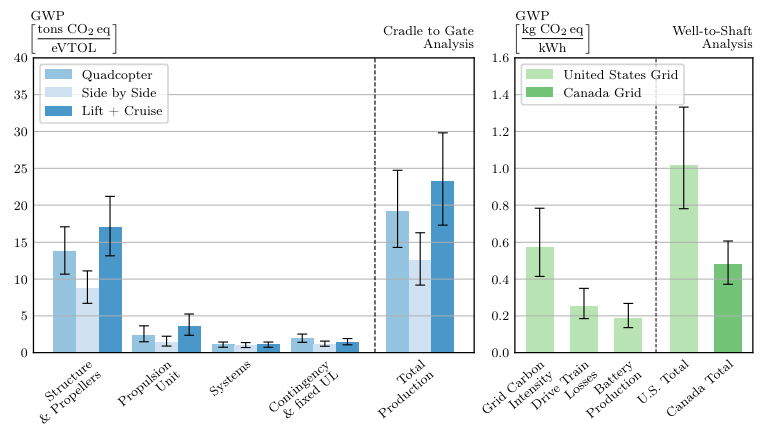
\includegraphics[width=0.8\linewidth]{figures//Sustainability/Emissions}
    \caption{GHG Emissions due to the production of materials (left) and due to the consumption of electric energy during operation (right). Quadcopter, side by side, and lift + cruise refer to different eVTOLs concepts. \cite{andre2019robust}}
    \label{fig:emissions}
\end{figure}


Additionally, looking at the analysis performed on different eVTOLs (\Cref{fig:emissionsspeed} \cite{andre2019robust}), a very clear dependency of the emissions on the velocity can be seen.
For all concepts, the minimum emissions speed is recorded between 150 km/h and 200 km/h.
The \textit{Swing}’s cruise speed of 200 km/h is thus very close to the optimal speed for minimising (GWP). This efficiency in operation further reduces the overall environmental impact during the vehicle's lifecycle.

\begin{figure}[h]
    \centering
    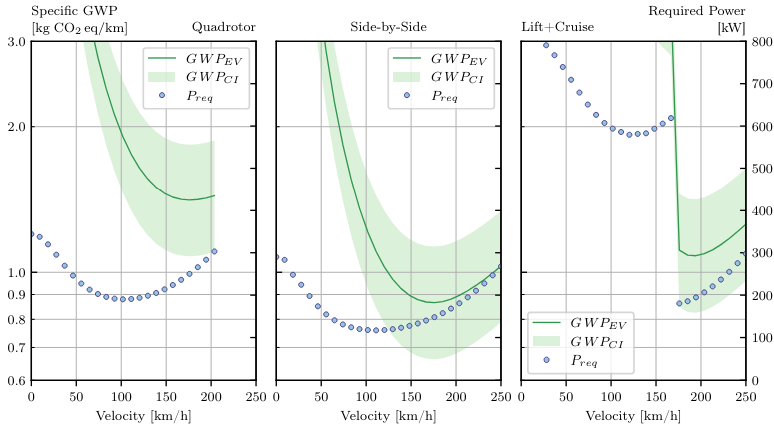
\includegraphics[width=1\linewidth]{figures//Sustainability/EmissionsSpeed}
    \caption{Powers (blue dots) and distance-specific emissions (green lines) over forward flight speed for the three eVTOL concepts. A 95\% confidence interval (CI) is indicated together with the mean (EV) \cite{andre2019robust}.}
    \label{fig:emissionsspeed}
\end{figure}


\section{Reusability of Vehicle Parts: the \enquote*{Cradle to Cradle} Approach}
\label{sec:reusability}
Committing to sustainability, the \textit{Swing} not only aims to revolutionise urban transportation but also to set new standards for the reusability of its components.
Embracing the \enquote*{cradle to cradle} approach, as opposed to the traditional \enquote*{cradle to grave} concept,
we are dedicated to ensuring that every part of the vehicle can be repurposed or recycled,
minimising waste and environmental impact.

\subsection*{Partnerships for Component Repurposing}
Partnerships are planned with industry leaders such as Tarmac Aerosave and Satir, known for their expertise in aircraft component recycling and repurposing.
These collaborations will enable the effective management of the end-of-life cycle of the \textit{Swing}, ensuring that its parts are given a second life.
By working with these companies, components can be disassembled, repurposed,
and recycled; thereby significantly reducing the environmental footprint of the vehicles.

Additionally, inspired by initiatives like the Lufthansa Upcycling Collection and Airbus’ A Piece of Sky, we are launching our homeware collection, \enquote*{\textit{Swing} Reimagined}.
This collection will feature unique items made from repurposed parts of the \textit{Swing}, offering our customers a chance to own a piece of aviation history while promoting sustainability. \Cref{fig:reimaginedbookshelf,fig:reimaginedswing} show some example pieces part of the \textit{Swing} Reimagined Collection.

\begin{figure}[h]
    \centering
    \begin{subfigure}[b]{0.49\textwidth}
        \centering
        
\includegraphics[width=1\linewidth]{figures/Sustainability/openart-image_9xYWF8B4_1718783125781_raw}
         \caption{CFRP wing skin structure repurposed as a bookshelf. [OpenAI generated image]}
        \label{fig:reimaginedbookshelf}
    \end{subfigure}
    ~
    \begin{subfigure}[b]{0.49\textwidth}
        \centering
        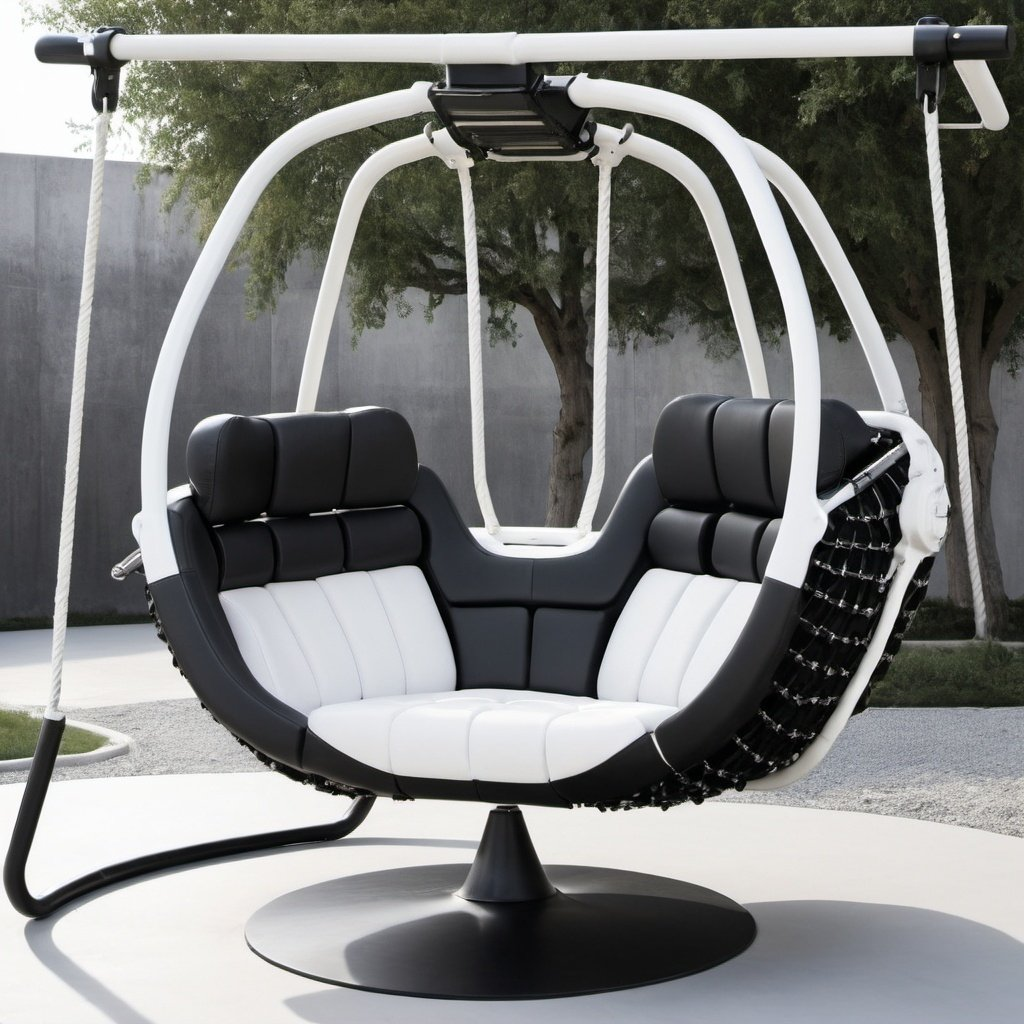
\includegraphics[width=1\linewidth]{figures/Sustainability/openart-image_bgvoo72x_1718783206289_raw}
         \caption{Front fuselage structure and seats repurposed as a comfortable Swing [OpenAI generated image]}
        \label{fig:reimaginedswing}
    \end{subfigure}
    \caption{Swing reimagined collection}
    \label{fig:reimagined_collection}
\end{figure}



\subsection*{Tactics to Facilitate the Repurposing Process}
To maximize the reusability and recyclability of our vehicle components, several key strategies are adopted:
\begin{itemize}
    \item Modularity: by designing the \textit{Swing} with a modular structure, we ensure that its components can be easily disassembled and reassembled.
    This facilitates the repurposing process and allows for straightforward upgrades and maintenance.

    For instance, the batteries are modular, allowing for the replacement of individual modules rather than the entire battery system in the event of a failure.
    Moreover, the batteries are strategically placed in the nacelles rather than the wings, simplifying maintenance and replacement procedures.
    
    \item Standardisation: implementing standardised components and interfaces ensures compatibility with future technologies and systems.
    This not only simplifies repairs and replacements but also enhances the longevity and adaptability of the vehicle.
\end{itemize}


\subsection*{Recycling Goals and Industry Standards}
According to the Aircraft Fleet Recycling Association (AFRA), it is estimated that around 80\% to 85\% of aircraft parts are recycled when an aircraft reaches retirement.
Our goal is to exceed this standard by aiming to recycle close to 95\% of the \textit{Swing}'s components.
By striving for this ambitious target, we demonstrate our commitment to leading the industry in sustainable practices and setting a benchmark for future developments in urban air mobility.

\subsection*{Long-Term Reusability Requirements}
We have set stringent requirements for the reusability of our vehicle to ensure long-term sustainability.
Specifically, requirements Co-4-STK13-1-5 and Co-4-STK13-1-6 guide our design and production processes.
Requirement Co-4-STK13-1-6 states: \enquote*{The vehicle structure shall be reusable for at least 10 years after its life.}
This ensures that the core components of the \textit{Swing} are built to last, further enhancing the vehicle’s sustainability credentials.

\section{Economic Sustainability of the \textit{Swing} Project}
Beyond its technological and operational benefits, the \textit{Swing} project promises substantial economic sustainability by positively impacting the local economy in several key ways.

Firstly, the \textit{Swing} project will create numerous job opportunities in both the manufacturing and operational sectors. Establishing production facilities for the \textit{Swing} will boost local employment rates by generating manufacturing, assembly, and quality control jobs. Additionally, the ongoing need for regular maintenance and operational support will create further employment in technical services, ground operations, and customer support.

Secondly, the \textit{Swing} will enhance mobility and connectivity, significantly benefiting the local economy. By providing efficient and rapid transportation, the \textit{Swing} improves access between urban and rural areas, facilitating easier access to jobs, education, healthcare, and other essential services. This enhanced connectivity allows for greater economic integration, enabling businesses to expand their markets and workforce and stimulating economic activity and growth.

Finally, the \textit{Swing} can potentially boost tourism and commerce within the region. Its capability to offer quick and convenient transportation can attract more tourists, making travel between attractions and cities more accessible. For business professionals, the \textit{Swing} provides a fast and efficient mode of travel, promoting increased business interactions and commerce, further stimulating the local economy.






